\section{Method}
\definecolor{lightblue}{rgb}{0.63, 0.74, 0.78}
\definecolor{seagreen}{rgb}{0.18, 0.42, 0.41}
\definecolor{orange}{rgb}{0.85, 0.55, 0.13}
\definecolor{silver}{rgb}{0.69, 0.67, 0.66}
\definecolor{rust}{rgb}{0.72, 0.26, 0.06}

\colorlet{lightsilver}{silver!30!white}
\colorlet{darkorange}{orange!75!black}
\colorlet{darksilver}{silver!65!black}
\colorlet{darklightblue}{lightblue!65!black}
\colorlet{darkrust}{rust!85!black}

\tikzstyle{trainingstyle} = [rectangle, 
minimum width=2cm, 
minimum height=2cm,
text centered,
text width=1.5cm,
draw=black,
thick,
rounded corners=0.3cm, 
fill=lightsilver, label=(a)]


\tikzstyle{onnxstyle} = [rectangle, 
minimum width=2cm, 
minimum height=0.8cm, 
text centered,
draw=black, 
thick,
rotate=90,
rounded corners=0.3cm,
fill=lightsilver, label=right:(b)]

\tikzstyle{mtestyle} = [rectangle, 
minimum width=2.7cm, 
minimum height=0.8cm, 
text centered, 
text width=2.8cm,
thick,
draw=black, 
rotate=90,
thick,
rounded corners=0.3cm,
fill=lightsilver, label=right:(d)]

\tikzstyle{decodingstyle} = [rectangle, 
minimum width=2cm, 
minimum height=0.8cm, 
text centered,
draw=black,
rotate=0,
thick,
rounded corners=0.3cm,
fill=rust!30, label=(f)]

\tikzstyle{eucstyle} = [rectangle, 
minimum width=2cm, 
minimum height=1cm,
text centered,
text width=1.55cm,
draw=black,
thick,
rounded corners=0.3cm, 
fill=white, label={[xshift=0.15cm]right:(g)}]

\tikzstyle{border1style} = [rectangle, 
minimum width=2.5cm, 
minimum height=4.75cm,
text centered,
text depth=4cm,
draw=black,
rounded corners=0.3cm, 
thick,
fill=lightsilver,
fill opacity=1, label={[xshift=0.5cm]above:(e)}]

\tikzstyle{border2style} = [rectangle, 
minimum width=4.5cm, 
minimum height=4cm,
text centered,
text depth=3.5cm,
draw=black,
dashed,
very thick,
rounded corners=0.3cm, 
fill=seagreen,
fill opacity=0.1,
text opacity=1,
label=(c)]

\tikzstyle{hpcstyle} = [rectangle, 
minimum width=2cm, 
minimum height=2cm,
text centered,
text width=1.9cm,
draw=black,
thick,
rounded corners=0.3cm, 
fill=lightsilver, label=(h)]

\tikzstyle{arrow} = [very thick,->,>=latex]
\tikzstyle{darrow} = [very thick,<->,>=latex]
    
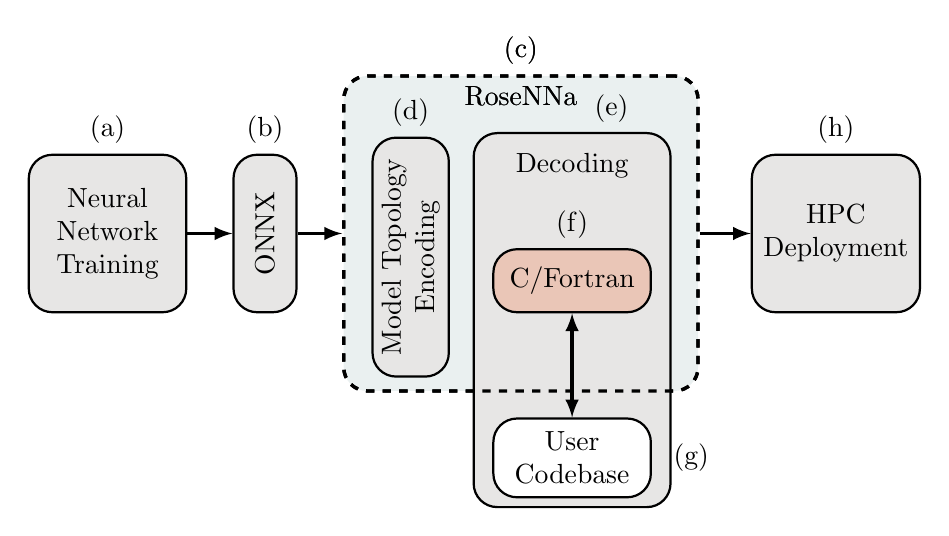
\begin{tikzpicture}[node distance=1cm]
\node (training) [trainingstyle] {Neural Network Training};

\node (onnx) [onnxstyle, below of=training, yshift=-1cm] {ONNX};

\node (border2) [border2style, right of=onnx, xshift=2.25cm,yshift=0cm] {RoseNNa};

\node (mte) [mtestyle, below of=border2, yshift=2.4cm, xshift=-0.3cm] {Model Topology \\ Encoding};

\node (border1) [border1style, right of=mte, xshift=1.05cm, yshift=-0.8cm] {Decoding};

\node (decoding) [decodingstyle, below of=border1,xshift=0cm,yshift=1.5cm] {C/Fortran};

\node (euc) [eucstyle, below of=decoding, yshift=-1.25cm] {User \\ Codebase};

\node (hpc) [hpcstyle, right of=border2, xshift=3cm, yshift=0cm] {HPC \\ Deployment};

\node (border2) [border2style, right of=onnx, xshift=2.25cm,yshift=0cm, fill=none] {RoseNNa};

\draw [arrow] (training) -- (onnx);
\draw [arrow] (onnx) -- (border2);
% \draw [arrow] (mte) -- (3.55,0);
\draw [darrow] (decoding) -- (euc);
\draw [arrow] (border2) -- (hpc);
\end{tikzpicture}
% 给定任意dynamic NeRF和他的训练video数据,我们的任务是通过修改某一帧的2D RGB图像编辑4D NeRF的appearance,并且可以渲染时序和view一致的free viewpoint视频。
Given a dynamic NeRF and its training video data, our task is to edit the local appearance of the dynamic NeRF by modifying a single 2D image in the training video.
%  that is temporally and multi-view consistent.
% To this end, we propose a framework that can edit the appearance of dynamic NeRF by 
% lifting the 2D edited content to a sequence of temporally consistent 3D edited content.
To this end, we propose a framework that can edit the appearance of dynamic NeRF 
by lifting the 2D edited content to a sequence of temporally consistent 3D edited content, as illustrated in~\figref{pipeline}.
% 我们先简短介绍dynamic NeRF 用来建模动态场景in sec, 
% 然后我们介绍我们设计的local surface representations在sec1介绍
We first briefly introduce dynamic NeRFs for modeling dynamic scenes and our problem setting in~\secref{dynerf}.
Then, we describe a local surface representation in~\secref{local_surface}.
% 同时,为了保证时序 consisent,我们提出了一种deformation representations,which 可以让我们的local surface trackable。
Meanwhile, we propose a motion representation that allows for the tracking of the local surface in~\secref{deformation}.
% 通过我们提出的local surface representations和deformation representations,我们可以恢复出(a deformation sequence of local surface with the non-rigid surface motion), 有利于对于local surface上的点加上explicit约束。
Next, \secref{reg} describes our training losses for the motion representation and the constraints that are applied to the local surface.
Finally, \secref{editing} illustrates how to render edited results after training.

\subsection{Preliminary}
\label{dynerf}
% 下文我们就将能够表示动态场景的神经辐射场的方法统称为dynamic NeRF。
\paragraph{Dynamic NeRFs.}
In this paper, we use the term ``dynamic NeRF'' to refer to the neural radiance fields that can represent dynamic scenes.
% 现有的动态NeRF将场景表示为一个时变的连续神经辐射场,即一个从空间位置$\mathbf{x}$,时间$t$,和viewing direction $\mathbf{d}$到颜色和密度的映射。
Existing dynamic NeRFs~\cite{park2021nerfies, peng2021neural, park2021hypernerf,Gao2021DynNeRF,li2022neural,li2020neural} represent dynamic scenes as a time-varying continuous neural radiance field,
i.e., a mapping function $f_\theta$ from a spatial position $\mathbf{x}$, time $t$, and viewing direction $\mathbf{d}$ to color and density.
% 可以表示成如通用的公式:
It can be represented as a general equation:
\begin{equation}
    f_\theta:\left(\mathbf{x} \in \mathbb{R}^3, t \in \mathbb{R}, \mathbf{d} \in \mathbb{S}^2\right) \mapsto\left(\sigma \in \mathbb{R}^{+}, \mathbf{c} \in \mathbb{R}^3\right).
\end{equation}
% 不同dynamic NeRF对于modeling of time-varying scene content不一样。
Different dynamic NeRFs have different ways of modelling time-varying scene content.
% 一些works~\cite{Gao2021DynNeRF,li2020neural}采用了一个an additional ‘time coordinate’输入MLPs来表示场景动态变化。
Some works~\cite{Gao2021DynNeRF,li2020neural} adopt MLPs taking an additional ``time coordinate'' as input to represent the dynamic components of the scene.
% Nerfies~\cite{park2021nerfies}使用了一系列时间变化的形变场表示场景随时间的变化。
Nerfies~\cite{park2021nerfies} uses a series of time-varying deformation fields to represent the change of scene over time.
% Neural Body~\cite{peng2021neural}通过一个时间变化的人体参数模型来表示场景动态内容。
Neural Body~\cite{peng2021neural} represents the dynamic content of the scene by a time-varying human parametric model.
% 我们的方法对于dynamic NeRF表示agnostic,我们的方法可以和大部分dynamic NeRF结合。
Our method is designed to be compatible with most dynamic NeRFs.

\paragraph{Problem setting.}
Our goal is to edit the appearance of the given dynamic NeRF $f_\theta$ by modifying a single 2D image in the training video  $\{\mathbf{I}_i\}^N_{i=1}$, 
and then render a free-viewpoint video that is temporally consistent and high-quality.
For convenience, we refer to the image that the user wants to edit as the reference image. 
%  我们的方法既可以在单目数据上训练,也可以在多目数据上训练。$N_v$代表相机的个数。
Our method can be trained on both monocular and multi-view data. $N_v$ denotes the number of cameras.

% 在这里,我们假设想要编辑区域在大部分情况下可以被观测到没有被遮挡。并且我们只假定用户只编辑图片中的部分区域,而不是如风格化那种编辑全图。
We assume that the region to be edited can be observed without occlusion in most cases.
Additionally, we assume that the user only edits part of the image, rather than the entire image.

\subsection{Local Surface}
\label{local_surface}
% Although dynamic NeRFs can reconstruct complex dynamic scenes,
% 在单张编辑的图片上finetune NeRF,然后编辑NeRF的外观。
% it is difficult to edit the appearance of dynamic NeRFs by finetuning on a single image.
% This is because NeRFs do not have a well-defined surface.
% After editing, the rendered image in other views will have artifacts such as blurring and distortion.
% Similar problem is also discussed in NeuMesh~\cite{yang2022neumesh}.
% Similar problems are also discussed in NeuMesh~\cite{yang2022neumesh}.
% 如果我们有一个好的表面模型,我们就可以通过单张图片编辑表面模型的外观,并且能够保证view consistency。
% If we have a well-defined surface model, we can edit the appearance of the surface model using a single image,
%  which is able to guarantee view consistency.
% 例如,在一个视角编辑mesh的外观,然后通过mesh渲染器渲染出来的图片在其他视角下也是一致的。
% For example, editing the appearance of the mesh in a certain view, and the rendered image produced by the mesh renderer is also consistent in other views.
% 然而从dynamic scene重建全局的表面模型是一个很难的问题, 因为动态场景存在复杂的运动和遮挡,特别有些动态重建任务可能只有比较少的观测视角。
% However, reconstructing the global surface model for  dynamic scenes is a challenging problem,
% due to the complex motion and occlusion in dynamic scenes, 
% especially for some dynamic reconstruction tasks that may only have a few observation views.
% 我们观察到对于从单张图片编辑NeRF的任务具有local的特点,即用户通常只需要编辑图片中的一部分,而不需要编辑整个图片。
% We observe that the task of editing NeRF from a single image has a local property, 
% i.e., users usually only need to edit a part of the image, rather than the entire image.
% it is difficult to edit the appearance of dynamic NeRFs by finetuning on a single image.
It is difficult to edit the appearance of dynamic NeRFs by finetuning them on a single image.
% 这是因为只在一张编辑图上优化dynamic NeRF容易让dynamic NeRF过拟合。
This is because optimizing dynamic NeRFs on a single image tends to cause overfitting problems.
% 我们观察到,对于local的编辑appearance任务来讲,大部分3D区域都是不需要编辑的,因此不需要让所有的3D区域都能在单张图片上训练。
% 然而most dynamic NeRFs使用一个MLP表示整个空间,这样的representation是global的,因此finetune local区域也会影响到其他区域。
Most dynamic NeRFs use an MLP to represent the entire space, thus finetuning their local regions will also affect other regions.
% 这种property使得现有的dynamic NeRFs很难适用local editing结合。
For local appearance editing tasks, we observe that most 3D regions do not need to be edited. 
% 我们只需要设计一个local layer插入到dynamic NeRF中,这样我们就可以只编辑local layer的参数,而不会影响到其他区域。
% Therefore, we only need to design a local layer to be inserted into the dynamic NeRF, 
% so that we can only edit the parameters of the local layer without affecting other regions.
Hence,  we only need to design a local layer to be inserted into the dynamic NeRF. By doing so, we can solely modify the parameters of this local layer, ensuring that other regions remain unaffected.
Motivated by this, we propose a plug-and-play local surface representation to edit the appearance of dynamic NeRFs.
% 我们的local surface representation使用了mesh-based surface representation可以容易地被建立
Our local surface representation adopts a mesh-based surface representation that can be easily constructed.
% 并且,我们通过设计让我们的表面representation可以很好的和dynamic NeRF的volume rendering结合。
Moreover, we design our surface representation to be compatible with the volume rendering equation to handle occlusion.
% 为了方便起见,我们将用户想要编辑的图像称为reference 2D image。
% 为了产生这个local surface,我们先用4D NeRF渲染reference 2D image对应的depth map。
To generate the local surface, we first render the depth map for the reference image using the given dynamic NeRF.
% 然后将用户想要编辑的区域将通过反投影变成mesh $S_r$ based on the predicted depth map。
Then, we unproject the user-edited region of the reference image back to 3D space to form the mesh, similar to Shih~\etal~\cite{Shih3DP20}.
% 具体来说,我们将每个用户编辑的pixel \mathbf{p}_i 反投影回3D空间 in world coordinates 形成mesh的vertices \mathbf{V_r}, 见下面的公式:
Specifically, we unproject user edited pixels $\{\mathbf{p}_i\}^K_{i=1}$ back to 3D space in world coordinates to form the vertices $\{\mathbf{v}_r^i\}^K_{i=1}$ of the mesh, as shown in~\equref{unproject}:
\begin{equation}
\{\mathbf{v}_r^i\}^K_{i=1} = \mathbf{M}_{c2w} \Pi^{-1}(\{\mathbf{p}_i\}^K_{i=1}),
\label{unproject}
\end{equation}
%  \Pi^{-1}(\mathbf{p}_i) represents the inverse perspective projection operation applied to the 2D image point. \mathbf{M}_{c2w} is the camera-to-world transformation matrix,
% 用来将mesh vertices从camera coordinates转换到world coordinates。
where $\Pi^{-1}$ represents the inverse perspective projection operation. $\mathbf{M}_{c2w}$ is the camera-to-world transformation matrix, 
which is used to transform the mesh vertices from camera coordinates to world coordinates.
$K$ is the number of mesh vertices. 
% 相邻的pixel变成的vertices相连就可以形成mesh的face
The vertices of neighboring pixels are connected to form the faces of the mesh.

% 我们也定义了mesh的每个vertex的color为reference 2D image中对应pixel的颜色。
We define the color of each vertex of the mesh as the color of the corresponding pixel in the reference image.
% 对于一个ray上的任意一个点来讲,他们的color基于射线与三维网格的交点所在面的顶点颜色,通过使用重心坐标的加权和进行插值计算得到的。
% 在渲染mesh的时候,我们对每条ray上的点都手工定义颜色
When rendering the mesh, we manually define the color for each point along the ray.
For any point on the rays intersecting the mesh, its color $\mathbf{c}^s$ is calculated by interpolating the vertex colors of the intersecting face of the 3D mesh using barycentric coordinates as weights.
%对于没有和mesh先交 
For any point on the rays that does not intersect the mesh, its color $\mathbf{c}^s$ is set to zero.

% Although the local surface representation is easy to construct, 
% it is difficult to 和original dynamic NeRF处理遮挡关系。
Although the local surface representation is easy to construct,
it is difficult to handle occlusion relationships between the local surface and the original dynamic NeRF, as shown in~\figref{occ}.
% 为了处理遮挡关系,我们设计的surface表示能够和给定的dynamic NeRF一起通过volume rendering渲染.
% To tackle this problem, our surface representation is designed to be compatible with the given dynamic NeRF for volume rendering.
To address this problem, we  design our surface representation to be seamlessly integrated with the given dynamic NeRF for volume rendering.
% 我们将mesh转换成distance field根据空间中的点到mesh的最近距离
We convert the mesh into a distance field according to the nearest distance from a point to the mesh.
% 然后再转换成density field。
Then, the distance field is converted into a density field.
% 受到volsdf的启发,我们使用下面方程将distance field转换成density field。
Inspired by VolSDF~\cite{yariv2021volume}, we convert the distance field into the density field using~\equref{volsdf}:
\begin{equation}
    \sigma^d(\mathbf{x})=\alpha \Psi_\beta\left(-d(\mathbf{x})\right),
    \label{volsdf}
\end{equation}
% where $\alpha=\beta^{-1}$ and $\beta$ are 手工定义的 parameters
where $\alpha=\beta^{-1}$, $\beta$ is a 
 manually defined parameter, 
$d(\mathbf{x})$ is the distance from the mesh to the point $\mathbf{x}$,
% $\Psi_\beta$ is the CDF of the Laplace distribution with zero mean and a scale of $\beta$.
and $\Psi_\beta$ represents the cumulative distribution function of the Laplace distribution with zero mean and a scale of $\beta$.
% 为了让surface替换掉原本nerf的区域让local surface不影响其他区域,我们定义一个的mask field,用来表示空间中的区域属于local surface还是dynamic NeRF。
To ensure that the local surface replace the original dynamic NeRF in the edited region 
and does not affect other regions of the dynamic NeRF,
we define a mask field to indicate which regions belong to the local surface and which regions belong to the dynamic NeRF.
% 对于距离surface gamma以内的区域为1距离gamma以外的区域为0
For points within a distance of $\gamma$ from the surface, the mask value is set to 1. For points beyond a distance of $\gamma$ from the surface, the mask value is set to 0.
% 如果一条ray并没有和mesh相交我们就将该ray上由surface产生的density全部置为0。
If a ray $\mathbf{r}(t)$ does not intersect with the mesh, we set the mask value to 0 for all points on the ray.
The mask field is defined as:
\begin{equation}
M(\mathbf{x}) = \begin{cases}
    1, & \text{if $ d(\mathbf{x}) < \gamma$ and $\mathbf{r}(t) \in \mathcal{R}_h$} \\
    0, & \text{otherwise}
\end{cases},
\label{mask}
\end{equation}
where $\mathcal{R}_h$ is the set of all rays that intersect with the mesh.
% 最后的volume rendering 公式为:
Our ultimate volume rendering equation is:
\begin{equation}
    \mathbf{C}^{full}(\mathbf{r})=\sum_{i=1}^N T_i^{full}\left(\alpha\left(\sigma_i^d \delta_i\right)(1-M_i) \mathbf{c}_i^d+\alpha\left(\sigma_i^s \delta_i\right) M_i \mathbf{c}_i^s\right),
    \label{volume}
\end{equation}
where $\mathbf{C}^{full}$ is the rendered color of the ray $\mathbf{r}$ and
$\alpha(x)=1-\exp \left(-x\right)$.
$\sigma^d$ and $\sigma^s$ are the densities of the dynamic NeRF and the local surface,
$\delta$ is the distance between adjacent sample points.
$M_i$ is the mask value at the $i$-th sample point. $\mathbf{c}^d$ and $\mathbf{c}^s$ are the colors of the dynamic NeRF and the local surface.
$T_i^{full} = \exp(-\sum_{j=1}^{i-1} (\sigma_j^d \delta_j (1-M_j) + \sigma_j^s \delta_j M_j))$
is the accumulated transmittance of the ray $\mathbf{r}$ up to the $i$-th sample point.

\subsection{Motion Representations}
\label{deformation}
% 通过上面的方法,我们仅仅生成了某一帧的local surface,其他帧的local surface位置还不确定,
Through the above method, we only generate the local surface of a certain frame.
The positions of the local surface of other frames are still unknown.
% 所以我们需要将local surface传播到其他帧下。
Therefore, we propose our motion representation to propagate the local surface to other frames.
% 为了将local surface传播到其他帧下,受到CaDex的启发,我们使用 invertible networks to model our scene motion.
Inspired by CaDeX~\cite{Lei2022CaDeX}, we use invertible networks to model our scene motion.
% invertible networks是严格的bijective map,比传统的两个MLP表示deformation Networ和inverse deformation Network的方法~\cite{tewari2022disentangled3d}更加fits the natural properties of non-rigid
%motion, as also shown in~\cite{Lei2022CaDeX, Cai2022NDR}
Invertible networks are strictly bijective maps, which fits the natural properties of non-rigid motion better than the traditional method~\cite{tewari2022disentangled3d} of using two MLPs to represent the deformation and the inverse deformation.
% 使用invertible networks的好处是我们可以知道任意两帧的空间中的点的对应关系。这样我们就可以直接将$\br{S_r}$ warp到其他帧下,如公式:
By leveraging the invertible network, we can know the point-to-point correspondence between arbitrary two frames, as shown in~\equref{invwarp}:
\begin{equation}
    \mathbf{x}_{t \rightarrow t'}=\mathcal{H}_{t'}^{-1} \circ \mathcal{H}_t\left(\mathbf{x}_t\right),
\label{invwarp}
\end{equation}
where $\mathcal{H}_t$ represents the operation of mapping the point $\mathbf{x}_t$ from the the observation space at frame $t$ to the canonical space by the invertible network,
and $\mathcal{H}_{t'}^{-1}$ is the inverse operation of mapping the point $\mathbf{x}_{t'}$ from the canonical space to the observation space at frame $t'$.

% 理论上来讲,我们可以采用如NSFF~\cite{li2020neural}训练相邻两帧之间scene flow fields一样的方法来让invertible networks学习到相邻两帧之间的对应关系。
Theoretically, we can train the invertible network to learn the correspondence between adjacent frames in the same way as NSFF~\cite{li2020neural}.
% 由于invertible networks是严格的bijective map,在学习完每个arbitrary相邻帧的对应关系后,我们可以知道任意两帧之间的对应关系.
Because the invertible network is a strictly bijective map, after learning the correspondence between each pair of adjacent frames,
the correspondence between any two frames is naturally known.
% 因为NSFF需要使用volume rendering将scene flows转化到2D相机平面上利用2D监督,然后使用temporal photometric consistency和data-driven priors监督scene flows的训练。
% However, this training strategy needs to use volume rendering to transform the scene flows into optical flows on the 2D image plane for 2D supervision.
However, this training strategy needs to 
densely sample the points in 3D space to transform the scene flows into optical flows on the 2D image plane for 2D supervision.
% 但由于invertible networks的显存占用太大了,
% 我们无法使用和上述volume rendering一样的方法来训练invertible networks。
Due to the large GPU memory consumption of the invertible network, 
we cannot use the same strategy as above to train the invertible network.
% 所以我们采用了一个MLP表示scene flow fields,和Gao~\etal一样,唯一不同的是我们不使用positional encoding编码空间位置信息,如公式:
To resolve this problem, we employ an MLP $f_\phi$ to model the scene flow field and then use $f_\phi$ to distill the motion information to the invertible network.
% , which is the same as~\cite{li2020neural, Gao2021DynNeRF}, 
% except that we do not use positional encoding to encode the spatial position information, as shown in~\equref{scene_flow}:
The MLP $f_\phi$ is defined as:
\begin{equation}
\left(\mathbf{f}_{t \rightarrow t+1}, \mathbf{f}_{t \rightarrow t-1}\right)=f_\phi(\mathbf{x}, \gamma(t)), 
\label{scene_flow}
\end{equation}
where $\mathbf{f}_{t \rightarrow t+1}$ and $\mathbf{f}_{t \rightarrow t-1}$ are the scene flow fields from frame $t$ to frame $t+1$ and frame $t$ to frame $t-1$,
 and $\gamma(t)$ is the positional encoding of $t$.
We adopt the loss function described in~\equref{invertible_networks} to train the invertible network and only sample training points near the local surface, which can greatly reduce memory consumption.
% 我们的scene flow fields和Gao~\etal的损失函数是一样的,详见补充材料。
%Our scene flow fields and the loss function are the same as~\cite{Gao2021DynNeRF}, which is shown in the supplementary material.
% 然后再将MLP学到的scene flow蒸馏给invertible networks,这样就可以让invertible networks学习到local surface每帧的三维空间位置,如公式:
% Then, we distill the scene flow fields learned by the MLP to the invertible networks, 
% so that the invertible networks can learn the spatial position of the local surface in each frame,
\begin{equation}
\mathcal{L}_{distill}=\sum_{\mathbf{x}\in \mathcal{X}_{surf}}(||\mathbf{f}_{t \rightarrow t+1}^{\mathrm{inv}}-\mathbf{f}_{t \rightarrow t+1}||+||\mathbf{f}_{t \rightarrow t-1}^{\mathrm{inv}}-\mathbf{f}_{t \rightarrow t-1}||),
\label{invertible_networks}
\end{equation}
where $\mathbf{f}_{t \rightarrow t+1}^{\mathrm{inv}} = \mathbf{x}_{t \rightarrow t+1} - \mathbf{x}_t$ and $\mathbf{f}_{t \rightarrow t-1}^{\mathrm{inv}} = \mathbf{x}_{t \rightarrow t-1} - \mathbf{x}_t$ 
are the scene flows predicted by the invertible networks. 
%在local surface附近的点
$\mathcal{X}_{surf}$ is the set of points near the local surface.
% 注意我们只在local surface上采样点训练invertible networks,这样可以非常减少显存占用。
\subsection{Training}
\label{reg}
We utilize the motion matching loss to supervise the scene flow field $f_\phi$:
\begin{equation}
\label{motion_matching_loss}
\mathcal{L}_{motion}=\sum_{\mathbf{r}\in \mathcal{R}} \sum_{j \in\{i \pm 1\}} || \hat{\mathbf{p}}_{i \rightarrow j}\left(\mathbf{r}_i\right)-\mathbf{p}_{i \rightarrow j}\left(\mathbf{r}_i\right) ||,
\end{equation}
where $\mathcal{R}$ is the set of rays, $\hat{\mathbf{p}}_{i \rightarrow j}$ 
is the ground truth optical flow from frame $i$ to frame $j$ predicted by RAFT~\cite{teed2020raft},
and $\mathbf{p}_{i \rightarrow j}$ is the optical flow induced by the scene flow $\mathbf{f}_{i \rightarrow j}$.
% 由于我们通过invertible networks建立任意两帧的空间点的对应关系,deformation sequence of our local surface可以被轻易恢复。

The deformation sequence of our local surface can be recovered easily through the invertible networks,
% 这让我们可以非常方便地在local surface上面加正则项以消除累积误差由scene流带来的
which allows us to easily add regularization terms on the local surface to eliminate accumulated errors caused by the scene flow.
% 我们介绍拉普拉斯光滑term和 feature-based photometric term在本section
We introduce the Laplacian smooth term and the feature-based photometric term as follows.
% 拉普拉斯光滑term是常用的用于让mesh更加smooth的正则项,如公式

The Laplacian smooth term is a common regularization term used to make the mesh more smooth, as shown in~\equref{laplacian_smooth}:
\begin{equation}
\mathcal{L}_{lap}=\sum_{\mathbf{v}^i \in \mathcal{V}}  \left\|\mathbf{v}^i_t-\mathbf{\bar{v}}^i_t\right\|^2 \text{, where } 
\mathbf{\bar{v}}^i_t = \sum_{j \in \mathcal{N}(i)} \mathbf{v}^j_t,
\label{laplacian_smooth}
\end{equation}
% where $\mathbf{V}$ is the set of vertices of the local surface,
where $\mathcal{N}(i)$ is the set of neighboring vertices of the $i$-th vertex, 
and $\mathbf{v}^i_t$ is the $i$-th vertex of the local surface at frame $t$. $\mathcal{V}$ is the set of all the vertices of the local surface.
% 我们直接使用了作为weight matrix.
% 为了让每一帧的surface与图像对齐,feature-based photometric term被用来衡量surface和图像的对齐程度,如公式:
To align the surface with the image in each frame, 
the feature-based photometric term is utilized to measure the alignment between the surface and the image,
as shown in~\equref{feature_based_photometric}:
\begin{equation}
\begin{aligned}
&\mathcal{L}_{pho}= \sum_{\mathbf{v}^i \in \mathcal{V}} \sum_{j=0}^{N_v}  s_{\cos }(F_{r}(\Pi(\mathbf{v}_r^i)), F^j_{t}(\Pi(\mathbf{v}_t^i))), \\
&    s_{\cos }(x, y)= max(1 - \frac{\langle x, y\rangle}{\|x\| \cdot\|y\|}, \epsilon),
\label{feature_based_photometric}
\end{aligned}
\end{equation}
where $F_{r}$ and $F_{t}$ are the features extracted from the reference image and the image at frame $t$,
$\Pi$ is the projection function  and $\mathbf{v}_r$ and $\mathbf{v}_t$ are the vertices of the local surface at the reference frame and frame $t$.
% $N_v$代表相机的数量.
$N_v$ is the number of cameras.
% $\epsilon$ 是一个阈值,用于防止遮挡导致不准确的监督信号。
$\epsilon$ is a threshold to prevent inaccurate supervision signals caused by occlusion.
% 我们采用s2d为这里的图像特征提取器,因为它能够提取出来的特征更加robust。
We adopt S2DNet~\cite{Germain2020S2DNet} as the feature extractor, for it can extract robust local features.
% 全部的losses在补充材料里。
Note that only $\mathcal{L}_{pho}$ may be supervised by multi-view images, while the other loss functions solely require supervision from single-view videos.
The complete loss functions are shown in the supplementary material.
% % 由于学习得到的scene flow比光流更容易累积误差,因此我们也对local surface添加光流一致性约束。
% Because the learned scene flow is more prone to accumulate errors than optical flow,
% we also add optical flow consistency constraints to the local surface.
% % 注意我们只对可见的顶点加这个约束,如公式:
% Note that we only add this constraint to the visible vertices, as shown in~\equref{optical_flow_consistency}:
% \begin{equation}
% \mathcal{L}^t_{opt}=\sum_{i=1}^{N}\sum_{j=1}^{M}||f_{t \rightarrow i}(\mathbf{S}_{t,i})-\mathbf{S}_{i,j}||,
% \label{optical_flow_consistency}
% \end{equation}
% where $f_{t \rightarrow i}$ is the optical flow from frame $t$ to frame $i$.
\subsection{Rendering Edited Results}
\label{editing}
% 在训练后,我们可以warp local surface到任意想要渲染的帧
After training, we can warp the local surface to any frame we want by the learned invertible networks. Then, we combine the local surface and the given dynamic NeRF, rendering them together according to~\equref{volume}. 
% 注意只有$\mathcal{L}_{pho}$可能会用多视角图片监督,其余的losses都只需要单视角video监督。


